% ---------------------------------------------------------------------------
% ---------------------------------------------------------------------------
% Modelo LaTex para preparação do documento final de Dissertação de Mestrado
% O modelo está em conformidade com ABNT NBR 14724:2011: 
% Programa de Pós-Graduação em Informática
% Universidade Federal do Rio de Janeiro
% Versão: v0.9
% ---------------------------------------------------------------------------
% ---------------------------------------------------------------------------

\documentclass[
	% -- opções da classe memoir --
	12pt,					% tamanho da fonte
	%openright,				% capítulos começam em pág ímpar (insere página vazia caso preciso)
	oneside,					% para impressão em verso e anverso. Oposto a oneside
	a4paper,					% tamanho do papel. 
	% -- opções da classe abntex2 --
	chapter=TITLE,			% títulos de capítulos convertidos em letras maiúsculas
	section=TITLE,			% títulos de seções convertidos em letras maiúsculas
	%subsection=TITLE,		% títulos de subseções convertidos em letras maiúsculas
	%subsubsection=TITLE,	% títulos de subsubseções convertidos em letras maiúsculas
	% -- opções do pacote babel --
	brazil,					% idioma adicional para hifenização
	%french,					% idioma adicional para hifenização
	%spanish,				% idioma adicional para hifenização
	english					% o último idioma é o principal do documento
	]{abntex2}

% ---------------------
% Pacotes OBRIGATÓRIOS
% ---------------------
\OnehalfSpacing
\usepackage{lmodern}				% Usa a fonte Latin Modern
%\usepackage{fontspec}
%\setmainfont{Arial}		
\usepackage[T1]{fontenc}			% Selecao de codigos de fonte.
\usepackage[utf8]{inputenc}		% Codificacao do documento (conversão automática dos acentos)
\usepackage{lastpage}			% Usado pela Ficha catalográfica
\usepackage{indentfirst}			% Indenta o primeiro parágrafo de cada seção.
\usepackage{color}				% Controle das cores
\usepackage{graphicx,graphicx}	% Inclusão de gráficos
\usepackage{epsfig,subfig}		% Inclusão de figuras
\usepackage{microtype} 			% Melhorias de justificação
\usepackage[top=3cm, bottom=2cm, left=3cm, right=2cm]{geometry}
% Estava assim: 2018-04-02
%\usepackage[top=3.1cm, bottom=2.2cm, left=3.1cm, right=2.2cm]{geometry}
%
% ---------------------
		
% ---------------------
% Pacotes ADICIONAIS
% ---------------------
\usepackage{lipsum}						% Geração de dummy text
\usepackage{amsmath,amssymb,mathrsfs}	% Comandos matemáticos avançados 
\usepackage{setspace}  					% Para permitir espaçamento simples, 1 1/2 e duplo
\usepackage{verbatim}					% Para poder usar o ambiente "comment"
\usepackage{tabularx} 					% Para poder ter tabelas com colunas de largura auto-ajustável
\usepackage{afterpage} 					% Para executar um comando depois do fim da página corrente
\usepackage{url} 						% Para formatar URLs (endereços da Web)
\usepackage{lscape}
\usepackage{multirow}
% ---------------------

% ---------------------
% Pacotes de CITAÇÕES
% ---------------------
\usepackage[brazilian,hyperpageref]{backref}	% Paginas com as citações na bibl
\usepackage[alf]{abntex2cite}				% Citações padrão ABNT (alfa)
%\usepackage[num]{abntex2cite}				% Citações padrão ABNT (numericas)
% ---------------------

\usepackage{pdfpages}

% testando criação de quadros na tese - 2018-04-02
% Novo list of (listings) para QUADROS

\newcommand{\quadroname}{Quadro}
\newcommand{\listofquadrosname}{Lista de quadros}

\newfloat[chapter]{quadro}{loq}{\quadroname}
\newlistof{listofquadros}{loq}{\listofquadrosname}
\newlistentry{quadro}{loq}{0}

% configurações para atender às regras da ABNT
\counterwithout{quadro}{chapter}
\renewcommand{\cftquadroname}{\quadroname\space} 
\renewcommand*{\cftquadroaftersnum}{\hfill--\hfill}

% Configuração de posicionamento padrão:
\setfloatlocations{quadro}{hbtp}

% fim testando criação de quadros na tese - 2018-04-02

% testando tabelas coloridas 2018-04-02
\usepackage[table]{xcolor}

% fim testando tabelas coloridas

% Configurações de CITAÇÕES para abntex2
% --- 
% CONFIGURAÇÕES DE PACOTES
% --- 

% ---
% Configurações do pacote backref
% Usado sem a opção hyperpageref de backref
\renewcommand{\backrefpagesname}{Citado na(s) página(s):~}
% Texto padrão antes do número das páginas
\renewcommand{\backref}{}
% Define os textos da citação
\renewcommand*{\backrefalt}[4]{
	\ifcase #1 %
		Nenhuma citação no texto.%
	\or
		Citado na página #2.%
	\else
		Citado #1 vezes nas páginas #2.%
	\fi}%
% ---

% Inclusão de dados para CAPA e FOLHA DE ROSTO (título, autor, orientador, etc.)
% ---
% Informações de dados para CAPA e FOLHA DE ROSTO
% ---
\titulo{Enhancing Depression Symptoms Diagnostic\\through Social Media Data}
\autor{Silas Pereira Lima Filho}
\local{Rio de Janeiro}
\data{2019}
\orientador{Jonice de Oliveira Sampaio, Dsc.}
\instituicao{%
  Universidade Federal do Rio de Janeiro
  \par
  Instituto de Matemática
  \par
  Instituto Tércio Pacitti de Aplicações e Pesquisas Computacionais
  \par
  Programa de Pós-Graduação em Informática}
\tipotrabalho{Tese (Doutorado)}
% O preambulo deve conter o tipo do trabalho, o objetivo,
% o nome da instituição e a área de concentração
\preambulo{\textbf{Qualificação de Doutorado} apresentada ao Programa de Pós-Graduação em Informática, Instituto de Matemática e Instituto Tércio Pacitti da Universidade Federal do Rio de Janeiro(área de concentração: Sistemas de Informação), como parte dos requisitos necessários para a obtenção do Título de Doutor em Informática.}
% ---

% Inclui Configurações de aparência do PDF Final
%  Configurações de aparência do PDF final
% NÃO ALTERAR!!!

% alterando o aspecto da cor azul
\definecolor{blue}{RGB}{41,5,195}

% informações do PDF
\makeatletter
\hypersetup{
     	%pagebackref=true,
		pdftitle={\@title}, 
		pdfauthor={\@author},
    		pdfsubject={\imprimirpreambulo},
	    pdfcreator={LaTeX with abnTeX2},
		pdfkeywords={abnt}{latex}{abntex}{abntex2}{trabalho acadêmico}, 
		colorlinks=true,       		% false: boxed links; true: colored links
    		linkcolor=black,          	% color of internal links
    		citecolor=black,        		% color of links to bibliography
    		filecolor=black,      		% color of file links
		urlcolor=blue,
		bookmarksdepth=4
} 
\makeatother
% --- 

% O tamanho da identação do parágrafo é dado por:
\setlength{\parindent}{2cm}

% Controle do espaçamento entre um parágrafo e outro:
\setlength{\parskip}{0.5cm}  % tente também \onelineskip

% ---------------------
% Compila o indice
% ---------------------
\makeindex
% ---------------------

%%%%%%%%%%%%%%%%%%%%%%%%%%%
%%  INICIO DO DOCUMENTO  %%
%%%%%%%%%%%%%%%%%%%%%%%%%%%
\begin{document}

% Retira espaço extra obsoleto entre as frases.
\frenchspacing

% ----------------------------------------------------------
% ELEMENTOS PRÉ-TEXTUAIS (Capa, Resumo, Abstract, etc.)
% ----------------------------------------------------------
\pretextual

% Capa
% ---
% Impressão da Capa
% ---
  \begin{capa}%
    \begin{figure}[h!]%
        \centering%
        
\includegraphics[width=\textwidth]{figs/banner.jpg}
      \end{figure}%
    \center
	\ABNTEXchapterfont\large{Universidade Federal do Rio de Janeiro\\ Instituto de Matemática\\Instituto Tércio Pacitti\\Programa de Pós-Graduação em Informática}
	%\vspace{1.2cm}

    \vfill
    \ABNTEXchapterfont\bfseries\LARGE\imprimirtitulo
    \vfill

	%\vfill
	\ABNTEXchapterfont\large\imprimirautor
	\vfill
%
	%úmero de Ordem PPGCC: M001
	
    \large\imprimirlocal
    \\\large\imprimirdata

    \vspace*{1cm}
  \end{capa}
% ---

% Folha de rosto (o * indica que haverá a ficha bibliográfica)
\imprimirfolhaderosto*

% Imprimir Ficha Catalografica
% ---
% Ficha Catalográfica
% ---
% Isto é um exemplo de Ficha Catalográfica, ou ``Dados internacionais de
% catalogação-na-publicação''. Você pode utilizar este modelo como referência. 
% Porém, provavelmente a biblioteca da sua universidade lhe fornecerá um PDF
% com a ficha catalográfica definitiva após a defesa do trabalho. Quando estiver
% com o documento, salve-o como PDF no diretório do seu projeto e substitua todo
% o conteúdo de implementação deste arquivo pelo comando abaixo:
%
% \begin{fichacatalografica}
%     \includepdf{fig_ficha_catalografica.pdf}
% \end{fichacatalografica}
\begin{fichacatalografica}
	\vspace*{\fill}					% Posição vertical
	\hrule							% Linha horizontal
	\begin{center}					% Minipage Centralizado
	\begin{minipage}[c]{12.5cm}		% Largura
	
	\imprimirautor
	
	EE74c\\   
    \hspace{0.5cm} \imprimirtitulo  / \imprimirautor. --
	\imprimirlocal, \imprimirdata-
	
	\hspace{0.5cm} \pageref{LastPage} f. \\%%: il. (algumas color.) ; 30 cm.\\
	
	\hspace{0.5cm} \imprimirorientadorRotulo~\imprimirorientador\\
    
%    \hspace{0.5cm}\imprimircoorientadorRotulo~\imprimircoorientador\\
	
	\hspace{0.5cm}
	\parbox[t]{\textwidth}{\imprimirtipotrabalho~--~\imprimirinstituicao,
	\imprimirdata.}\\
	
	\hspace{0.5cm}
		1. Depression Symptoms Identification.
		2. Complex Networks.
		3. Social Network Analysis.
		I. Oliveira, Jonice, Advisor
		II. Universidade Federal do Rio de Janeiro
		III. Enhancing Depression Symptoms Diagnostic through Social Media Data\\ 			
	
%	\hspace{8.75cm} CDU 02:141:005.7\\
	
	\end{minipage}
	\end{center}
	\hrule
\end{fichacatalografica}
% ---

% Inserir Folha de Aprovação
% ---
% Assinaturas
% ---
% Isto é um exemplo de Folha de aprovação, elemento obrigatório da NBR
% 14724/2011 (seção 4.2.1.3). Você pode utilizar este modelo até a aprovação
% do trabalho. Após isso, substitua todo o conteúdo deste arquivo por uma
% imagem da página assinada pela banca com o comando abaixo:
%
% \includepdf{folhadeaprovacao_final.pdf}
%
\begin{folhadeaprovacao}
	
	\begin{center}
		{\ABNTEXchapterfont\large\imprimirautor}
		
		\vspace*{\fill}\vspace*{\fill}
		\begin{center}
			\ABNTEXchapterfont\bfseries\Large\imprimirtitulo
		\end{center}
		\vspace*{\fill}
		
		\hspace{.45\textwidth}
		\begin{minipage}{.5\textwidth}
			\imprimirpreambulo
		\end{minipage}%
		\vspace*{\fill}
	\end{center}
	
	Trabalho aprovado. \imprimirlocal, DD de MMMM de 2019:
	
	\assinatura{\textbf{\imprimirorientador} \\ Orientador} 
%	\assinatura{\textbf{\imprimircoorientador} \\ Coorientador} 
	\assinatura{\textbf{Monica Ferreira da Silva, Dsc.} \\ UFRJ}
% 	\assinatura{\textbf{Marcos Roberto da Silva Borges, Dsc.} \\ UFRJ}
% 	\assinatura{\textbf{Renata Mendes de Araújo, Dsc.} \\ UNIRIO}
	%   \begin{center}
	%    \vspace*{0.1cm}
	%    {\large\imprimirlocal}
	%    \par
	%    {\large\imprimirdata}
	%    \vspace*{1cm}
	%  \end{center}
	
\end{folhadeaprovacao}
% ---

% Dedicatória
%% ---
% Dedicatória
% ---
\begin{dedicatoria}
   \vspace*{\fill}
   \centering
   \noindent
  % \textit{ Aos meus pais XXXXXXXX e YYYYYYY, \\ por sempre estarem comigo em todos os momentos.} \vspace*{\fill}
\end{dedicatoria}
% ---

% Agradecimentos
%% ---
% Agradecimentos
% ---
\begin{agradecimentos}

%Agradeço a Deus.\\
%\indent{Agradeço aos meus pais, XXXXX e YYYYY, por ...}

%Aos meus irmãos, por.....

%Agradeço ao meu orientador, XXXXXXXXX, por todos os conselhos, pela paciência e ajuda nesse período.

%Aos meus amigos ...

%Aos professores ...

%À XXXXXX pelo apoio financeiro para realização deste trabalho de pesquisa.

\end{agradecimentos}
%% ---

% Epígrafe
%% ---
% Epígrafe
% ---
\begin{epigrafe}
    \vspace*{\fill}
	\begin{flushright}
	%	\textit{``A educação tem raízes amargas, \\
    %              mas os seus frutos são doces.''\\
	%	          (Aristóteles)}
	\end{flushright}
\end{epigrafe}
% ---

% Resumo e Abstract
% ---
% RESUMOS
% ---

% RESUMO em português
\setlength{\absparsep}{18pt} % ajusta o espaçamento dos parágrafos do resumo
\begin{resumo}
% A inovação é um fator condicionante para o desenvolvimento organizacional, geração de riquezas e liderança de mercado. No cenário de mudanças recentes, nota-se um encurtamento do ciclo de vida dos produtos, cada vez mais condicionado aos desejos dos clientes e de tendências percebidas no mercado, exigindo respostas rápidas das organizações. Diante desse quadro, as startups vêm ganhando papel de destaque em função da flexibilidade do modelo de negócio, baixos investimentos iniciais e maior dinamicidade nos processos de transferência tecnológica. Como forma de viabilizar tais negócios, um número crescente de instituições de apoio tem se estabelecido para orientar empreendimentos nos seus primeiros dias. São investidores e capitalistas de risco, incubadoras e aceleradoras, além de órgãos governamentais de suporte – atores que compõem os ecossistemas de startups, provendo infraestrutura, espaço de mercado, parcerias consolidadas e processos estabelecidos. Essa comunidade empreendedora tão plural contribui em diferentes perspectivas para os novos empreendimentos, contudo traz uma série de desafios relacionados a convergência de interesses na rede. É fundamental para o ecossistema compreender quais são as competências, oportunidades e afinidades entre os membros para assegurar a harmonia e garantir a prosperidade do meio. 
%O presente trabalho apresenta um método para auxiliar no mapeamento dos recursos disponíveis, papel dos participantes, relações e comportamentos da comunidade baseado em métricas de  análise de redes sociais. Acredita-se que as respostas obtidas através deste estudo auxiliarão nos processos de tomada de decisões e na melhor compreensão das características e recursos disponíveis na rede.

 \textbf{Palavras-chaves}: Informática na Saúde Mental. Depressão. Análise de Redes Sociais. 
\end{resumo}

% ABSTRACT in english
\begin{resumo}[Abstract]
 \begin{otherlanguage*}{english}
% Innovation is a fundamental aspect of organizational development, wealth generation and market leadership. It has been noticed the shortening of the products lifecycle, which are much more conditioned by customer wishes and perceived market trends. It requires rapid responses from enterprises. Given this background, the lean startups have been gaining a prominent role due to the flexibility of the business model, low initial costs and greater dynamism in the technology diffusion. As a way to enable such businesses, a crescent number of support institutions have established to guide ventures in their early stages. They are made up of investors and venture capitalists, incubators and accelerators, as well as support government agencies - actors that compose the startup ecosystems, providing infrastructure, market space, consolidated partnerships and established processes. This heterogeneous entrepreneurial community contributes in different perspectives for these new firms. However it brings a series of challenges related to the convergence of interests in the network. It is critical for the ecosystem to understand the competencies, opportunities and affinities among members to take harmony and ensure the prosperity of the environment. This work presents a method to aid the identification and characterization of partnerships ties based on metrics of social network analysis. It is believed that the answers obtained through this study will help in the decision-making processes and the better understanding of the characteristics and resources available in the startup ecosystem.

   \vspace{\onelineskip}
 
   \noindent 
   \textbf{Keywords}: Mental Health Informatics. Depression. Social Network Analysis.
 \end{otherlanguage*}
\end{resumo}

% Lista de ilustrações
\pdfbookmark[0]{\listfigurename}{lof}
\listoffigures*
\cleardoublepage

% Lista de tabelas
\pdfbookmark[0]{\listtablename}{lot}
\listoftables*
\cleardoublepage

% Lista de abreviaturas e siglas
\begin{siglas}

  \item[ARS]\textit{Análise de Redes Sociais}
%   \item[ANPROTEC]\textit{Associação Nacional de Entidades Promotoras de Empreendimentos Inovadores}
%   \item[CEFET-RJ]\textit{Centro Federal de Educação Tecnológica do Rio de Janeiro}
%   \item[CMMI] \textit{Capability Maturity Model Integration}
%   \item[IETEC]\textit{Incubadora de Empresas Tecnológicas do CEFET/RJ}
%   \item[ReINC]\textit{Rede de Agentes Promotores de Empreendimentos Inovadores}
%   \item[TIC]\textit{Tecnologias da Informação e Comunicação}
  
\end{siglas}

% Lista de símbolos
%\begin{simbolos}
%  \item[$ \Gamma $] Letra grega Gama
%  \item[$ \Lambda $] Lambda
%  \item[$ \zeta $] Letra grega minúscula zeta
%  \item[$ \in $] Pertence
%\end{simbolos}

% Inserir o SUMÁRIO
\pdfbookmark[0]{\contentsname}{toc}
\tableofcontents*
\cleardoublepage

% ----------------------------------------------------------
% ELEMENTOS TEXTUAIS (Capítulos)
% ----------------------------------------------------------
\textual
% Elementos textuais com numeração arábica
\pagenumbering{arabic}
% Reinicia a contagem do número de páginas
\setcounter{page}{2}

% Inclui cada capitulo da Dissertação
%\include{capitulos/introducao}

% PARTE - Define a divisão do documento em partes (Não é obrigatório)
%\part{Preparação da pesquisa}
\chapter{Introduction}\label{cap:introduction}

% A criação de soluções inovadoras é uma das ações esperadas de uma abordagem científica. De forma geral e simplista, é através da observação de fenômenos, naturais ou artificiais, que o homem tenta entender um problema. Através de hipóteses, testes, validações e experimentações, o chamado cientista tenta apresentar soluções para os mais diversos problemas.
The creation of innovation solutions is one of the expectations from what is called scientific approach. In a simple and general way, it is from observation of phenomenas, natural or artifical one, that someone, normally called scientist try to discover new solutions for different problems and challenges.

% Em alguns momentos, os problemas abordados pelos cientistas são facilmente aplicáveis e a sociedade adjacente ao cientista consegue enxergar uma aplicação para o esforço científico. Deveras, é fato que o ser humano busca melhorar questões relacionadas à sua saúde mental ou física. Seja para estender a ``vida útil'' de uma pessoa com muita idade, ou então trazer bem estar para aquele que sofre com alguma patologia.
Ocasionally, tackled problems by researches are easilly appliable and the society who witness can visualize possible applications of that effort. Indeed, there is a wider effort which tries to improve solutions, and solve new problems related to mental and physical health. Since for extend the quality of life, for someone who suffers from any pathology.

Fato é que a saúde mental das pessoas tem sido discutida nos mais diversos círculos sociais e em diferentes mídias. Infelizmente, mais reportagens tem demonstrado que diferentes círculos sociais e econômicos são afetados por uma falta de tratamento e cuidado da saúde mental. A Classificação Estatística Internacional de Doenças e Problemas Relacionados com a Saúde, que está em sua décima versão (CID 10), padroniza os mais diversos tipos de doenças e patologias, de modo a que tal padronização ajude profissionais a identificarem os elementos que caracterizem determinada doença. Ele também classifica as diversas patologias em categorias, de modo hierárquico, agrupando assim doenças correlatas e similares.
The fact is that

% Depressão é uma das doenças mentais que mais recorrentes no mundo. Alguns dirão que é depressão é o mal do século. Em situações extremas, essa patologia pode levar a pessoa a ideação suicida e até mesmo ao ato em si \cite{AmericanPsychiatryAssociationApa2013}. A Organização Mundial da Saúde (OMS) apresenta o que cerca de 300 milhões de pessoas no mundo, de diferentes idades possuem algum nível de depressão\footnote{www.who.int/en/news-room/fact-sheets/detail/mental-disorders}. No Brasil, o Ministério da Saúde estima que 11,5 milhões de brasileiros são afetados pela depressão\footnote{www.blog.saude.gov.br/index.php/materias-especiais/52516-mais-de-onze-milhoes-de-brasileiros-tem-depressao}.
Depression is one of the most related mental diseases in the world. Some people call it the century illness due to its dangerousness. It can lead, in extreme situations, to suicide\cite{AmericanPsychiatryAssociationApa2013}. World Health Organization (WHO) presents a number of around 300 million people from different ages who suffer some kind of depression\footnote{www.who.int/en/news-room/fact-sheets/detail/mental-disorders}. Some of these symptoms are, for example, depressed mood in most of the day, lost of interest in regular activities, weight loss, and insomnia. In Brazil, the Health Ministry presents a number of 11,5 million people who are affected by depression \footnote{www.blog.saude.gov.br/index.php/materias-especiais/52516-mais-de-onze-milhoes-de-brasileiros-tem-depressao}. 

Em alguns momentos, depressão é erroneamente entendida como unicamente um estado emocional de tristeza. De fato alguém diagnosticado como depressivo tem o humor alterado. No entanto, a duração de tal estado do humor da pessoa é que diferirá alguém corretamente diagnosticado com a patologia depressão, de alguém que devido a algum acontecimento, está temporariamente triste ou cabisbaixa.
% Sometimes depression is wrongly understood as a emotional state which reflects sadness. Independently of above examples, the fact is that the mental disease depression is wrongly defined and acknowledged.
%Depression is one of the most related mental disease in the world and some people call it as the century illness. World Health Organization (WHO) presents a number of around 300 million people from different ages who suffer some kind of depression \footnote{www.who.int/en/news-room/fact-sheets/detail/mental-disorders}. 

%Depression is classified on 11th international Disease Classification (ICD 11) as a disease when it is diagnosed in someone behavior. Some of these symptoms are for example, depressed mood in most part of the day, lost of interest in regular activities, weight loss and insomnia. 
% Depression can happen triggered by an event where the person has lost something e.g. job, some close person etc.
%This disease is also dangerous in order of its extreme consequences. Depression, according to ICD 11, can lead to suicide ideation and consequently to suicide \cite{AmericanPsychiatryAssociationApa2013}.

%With the wide spread and with more people with depression, it becomes a challenge identify a person who can be in a real state of depression. Depression also afflicts people who are in specific location where the access to a professional is \textbf{costly impending}. Thus, identify and attend someone who could be a potential depressive patient, in a fast and unobtrusive way, seems very helpful. 

Segundo a OMS, a tendência é que cada vez mais pessoas sejam afetadas pela depressão. Por conta disso, é um desafio atender a um crescente número de pessoas que de fato sofrem tal doença, ou então que minimamente, possuem tendência a serem depressivas. Podemos listar desafios como, a formação de profissionais que atendam diretamente essas pessoas, ou então meios de diagnóstico prévio, meios de estreitar a comunicação entre profissional e cliente. Portanto, seria de grande ajuda, identificar e atender potenciais depressivos de modo rápido e não intrusivo.
% With more affected people, it becomes a challenge to identify a person who can be in a real state of major depression disease. It also afflicts people who are in a specific location where access to a professional is hindered due to cost. Thus, it is helpful to recognize and attend someone who could be a potential depressive patient, in a fast and unobtrusive way.

Sobre métodos de diagnóstico online, \cite{Horvitz} cita os termos \textit{infodemiologia} e \emph{detecção digital de doenças} como métodos correlatos que usam plataformas digitais e ferramentas de tecnologia para melhorar a saúde da sociedade. Esses termos podem ser entendidos como esforços para atacar a detecção de epidemias, indivíduos que estão em risco e também comunicar possíveis afetados por alguma doença. O uso de tecnologia poderia diretamente apoiar instituições, profissionais e também a própria população de forma geral. Fazendo assim com que as pessoas tenham conhecimentos sobre uma doença, e assim tornando-as mais conscientes sobre causas e sintomas de alguma doença.
% In the context of online diagnosis, \textit{infodemiology} and \textit{digital disease detection} are correlated terms to describe the use of digital platforms and tools to improve society health. They can be translated as efforts to tackle epidemics detection, identify individuals at risk, and communicate candidate urgent illness. The use of technology could directly support institutions, professionals, and even to aid people to make themselves aware of some disease\cite{Horvitz}.%, in order to allow aware inside society. In that way, people could be aware about some disease and its implications.
Sobre como identificar alguém com depressão, a Psicologia já possui métodos de diagnóstico e comumente é feito através de entrevistas do psicólogo com o paciente/cliente. Através dessa entrevista, o psicólogo identifica características no paciente que correlacionam com os sintomas da doença.
% Psychology already has methods to deal with depression identification. One of these methods is interview with psychologist. Through this conversation it could be possible to the professional, find some clues to identify someone with depression symptoms. 

% The abstraction of that is the question, how someone express himself? Some people might express through text, others will prefer with music, others will prefer to not externalize some feelings and sentiments about himself. This makes the task of identification more challenge.
% Nowadays, some groups of people have demonstrated an interesting behaviour. The act of express itself has been demonstrated on social media. People have express themselves more on these online platforms.  

Social media has been employed on academia to monitor people's behaviour and their personal choices. With this in mind, sounds interesting to investigate if it is possible to identify signs, symptoms of depressive behaviour on social media platforms.

As said above, the task of identifying some disease, even if it is not depression, can be challenging. Due to the plant offers of data types, select what is the most effective, precise and reliable technique, method analysis could require a great quantity of time of research.
 
Thus, we can abbreviate our effort as the following question: \emph{Is it possible to identify psychological diseases symptoms from people who are social media users?}
% . Recorte de interacoes de pessoas com sintomas de depressao em mídias sociais
% . Grupo de trabalhos sobre métricas e metodos de análise
Our research questions can be described as follow
\textit{It would be possible to identify psychological diseases symptoms using social media?}
% . Seria possivel identificar sintomas de doencas psicologicas por meio das midias sociais?	 
Is there a disturb diagnosis method only using data from social media? 


%As interações entre empresas distintas e outras entidades que colaboram entre si para compartilhar tecnologias, conhecimentos e trabalhar em conjunto são fundamentais para o desenvolvimento de novos produtos e serviços, fato corroborado por Ben Spigel \cite{spigel-2015}, que afirma que a inovação depende de um ambiente favorável para se desenvolver e potencializar a geração de outras mais, atraindo pessoas, recursos e oportunidades de fomento. 

%Esta rede de negócios tem sido analisada sob a ótica de ecossistemas, conforme inicialmente proposto por James F. Moore \cite{moore-1993}. A analogia estabelecida pelo autor procura estabelecer pontes das relações de parcerias entre os diferentes atores e o meio onde se inserem, considerando as mudanças constantes, como o surgimento de novos participantes, tecnologias e mercados e extinção de outros. Quando ocorrem de maneira integrada e dinâmica, possibilitam a evolução do ecossistema como um todo. 
%Em um ecossistema de startups, a comunidade é formada por empreendedores, apoiadores, universidades e outros grupos de interesse, que realizam atividades econômicas e negócios para estabelecer os meios necessários para lançar novos produtos no mercado \cite{lemos:2011, torres-souza:2016}. 

%As conexões em um ecossistema de startups são pautadas por dois tipos de interação: a colaboração e a competição. A colaboração é uma importante maneira de lidar com as incertezas inerentes do processo de inovação, através do compartilhamento dos riscos  \cite{chesbrough-appleyard:2007, west-bogers-2014}. 

%Além do mais, o sucesso de empreendimentos depende de um conjunto de infraestruturas e capacidades que abarcam desde a concepção do produto até a comercialização e distribuição no mercado. Frequentemente, as empresas consolidadas não controlam estes ativos complementares, no caso das startups, tal necessidade fica mais latente \cite{candido-souza-15}. 
%As relações de competição decorrem do princípio de que duas ou mais empresas possuem interesses divergentes onde uma empresa apenas obterá vantagem competitiva às custas de seus concorrentes. Este tipo de conexão, onde empresas cooperam em determinadas atividades e competem em outras é denominada \textquotedblleft coopetição\textquotedblright. A coopetição possui grande relevância para a geração de inovações e vêm motivando uma série de estudos que buscam compreender como pode ser gerenciado \cite{gubbins-dooley:2014, chesbrough-appleyard:2007, bengtsson-kock:2000}. 

%\textit{\textbf{outro importante fator ao abordar ecossistemas de startups é a coopetição - um modelo[?] onde empresas se organizam em estruturas de colaboração e por vezes competem entre si. }}

%O termo \textquotedblleft rede social online\textquotedblright\ é utilizado para descrever um grupo de pessoas que interage primariamente através de alguma mídia de comunicação. As redes sociais online têm facilitado a colaboração, o compartilhamento e a interação e tem aumentando a quantidade de informação de tal forma que existe muito mais informação sobre qualquer assunto do que uma pessoa seria capaz de absorver \cite{castells-96}.  Bevenuto e seus colegas \cite{bevenuto-2011} tratam rede social online como um serviço web que permite a construção de perfis públicos ou semi-públicos dentro de um sistema, a articulação de ações entre usuários que compartilham conexões.

%, tais como o grau de vértices, coeficiente de agrupamento, distância média, centralidade de nodos e reciprocidade,

\section{Problema}

%Para que funcionem de forma efetiva, é necessário entender como as relações são orquestradas. Neste sentido, uma série de paradigmas têm sido propostos para ampliar a compreensão das interações entre os diferentes atores das redes de inovação, tais como: o modelo da hélice tripla proposto por Etzkowitz \cite{etzkowitz:2008}, a estratégia de cocriação idealizada por Phahalad e Ramaswamy \cite{prahalad-ramaswamy-2004}, o modelo de ecossistemas de negócios, analogia criada por Moore \cite{moore-1993}.


%Conforme mencionado na Seção~\ref{sec:motivacao},

\section{Hipótese}
%A hipótese deste trabalho consiste na possibilidade de definição de um conjunto de técnicas para sistematizar o processo de análise e recomendação de parcerias em um ecossistema de startups através da Teoria de Grafos \cite{newman:2010}. A análise da rede visa a compreensão da dinâmica em que são firmadas ou extintas as conexões. Tal esforço possibilita a identificação de ações que possam aprimorar as relações, buscando a convergência de interesses para aumentar a resiliência do ambiente \cite{spigel-2015}. Para isto, consideram-se que os atores e as relações de parcerias existentes podem ser mapeadas como uma rede social heterogênea, onde diferentes atores possuem objetivos específicos no arranjo.

% A hipótese deste trabalho consiste na possibilidade de definição de um conjunto de métricas para auxiliar o processo de análise das relações de parcerias de um ecossistema de startups através da Teoria de Grafos \cite{newman:2010}. A análise da rede visa a compreensão da dinâmica em que são firmadas ou extintas as conexões, seus principais atores e possíveis ameaças. Tal esforço possibilita a identificação de ações que possam aprimorar as relações, buscando a convergência de interesses para aumentar a resiliência do ambiente \cite{spigel-2015}. Para isto, consideram-se que os atores e as relações de parcerias existentes podem ser mapeadas como uma rede social heterogênea, onde diferentes atores possuem objetivos específicos no arranjo.


%A hipótese deste trabalho se apresentará em duas partes. Na primeira, consideram-se que os atores e as relações de parceria existentes podem ser mapeadas como uma rede. A compreensão da dinâmica em que são firmadas ou extintas as conexões é fundamental para identificar ações que possam aprimorar as relações, buscando a convergência de interesses para aumentar a resiliência do ecossistema \cite{spigel-2015}. 

% Outra importante componente do estudo aborda a complementaridade necessária para cada participante do meio; \cite{west-bogers-2014} sugerem que há diferentes níveis de recursos externos compartilhados entre atores na busca por inovações. Cada participante da rede deve conhecer sua relevância frente a seus pares e que influências exerce \cite{easley-kleinberg:2010}. Desta forma, é preciso traçar estratégias de parceiras e identificar novos colaboradores que possam trazer novos recursos.  

% consiste na possibilidade de definição de um conjunto de técnicas que auxiliem na análise das parcerias existentes, recomendação de novas parcerias, identificação de conhecimentos desejáveis e as dependências na rede avaliação de relações de poder.

% Portanto, pretende-se utilizar as ferramentas de Análise de Redes Sociais para construir um modelo que, através de métricas estabelecidas, possa auxiliar nos processos de tomadas de decisões dos participantes do ecossistema de startup. Acreditamos que o mapeamento do cenário resultante possibilitará a identificação dos interesses envolvidos, os recursos disponíveis, as afinidades e aptidões da rede, possibilitando a recomendação de novos laços. 

%Em seguida, \textit{\textbf{[O uso de análise de redes sociais permitirá ao participante identificar que outros participantes podem trazer complementaridade para seus negócios, avaliar sua relevância na rede, seu poder de barganha e de influência, além de possibilitar traçar novos contatos para evitar dependências.]}}


\section{Objectives}
\label{sec:objectives}

Esta pesquisa tem ainda como objetivos específicos:

\section{Proposal Structure}
\label{sec:organization}
Este documento está estruturado da seguinte forma. O capítulo atual descreve a problemática abordada, e a hipótese que será abordada pela proposta de solução.
O Capítulo \ref{cap:depression} descreve a doença depressão sob o ponto de vista da psicologia, que é o campo de estudo apropriado.
O Capítulo \ref{cap:rev_literatura} apresenta o processo de mapeamento sistemático da literatura de forma a entender o atual estado da arte da computação para depressão.
No Capítulo \ref{cap:proposta}, é apresentada uma proposta de abordagem para identificar os sintomas da depressão numa mídia social. Sucessivamente, concluímos o documento no Capítulo \ref{cap:conclusao}.
\chapter{Depressão}\label{cap:depressao}

% Este capítulo apresenta os principais conceitos que fundamentam esta pesquisa. Para isto, foi feito uma revisão teórica sobre ecossistemas de startups e seus desdobramentos, contextualizando sua importância para o desenvolvimento de empreendimentos inovadores e para o contexto econômico atual.

\section{Inovação}

\begin{quote}
lorem ipslum
\end{quote}

\subsection{Gestão da Inovação}





\chapter{Revisão da Literatura}\label{cap:rev_literatura}

For the literature selection we have applied a systematic literature review in order to have a deeper insight from the most actual research which tackles the depression diagnosis in social media. 

From a computational perspective, the problem of dealing with depression and social media can be understand as search for people who suffer the symptoms of depression. Using different methods to identify if someone have depression or not, or if some person have one of the symptoms of depression. A good amount of articles relies on natural language processing (NLP) to make a systemic analysis over the text in social media publications.

In \cite{Zhao:2018:TCM:3302425.3302501}, the authors have applied text classification technique using Convolutional Neural Networks to classify depression using text analysis. The authors in \cite{Nobles:2018:IIS:3173574.3173987} also have used neural networks in order to find patterns on periods when the risk of suicide attempt is increasing in SMS texts. 

The work in \cite{Li2016} is a qualitative study that try to understand how is the behavior and reception of chinese population about depression. It is a qualitative study and differs from the prior ones.

De Choudhury is an author that we would like to highlight. She is one author who have developed many articles and researches about measurement of depression on social media context. Her works vary on some types of measurement and implications of depression in some contexts of affected persons. We will cite some of these works due to the importance and relevance of her effort to contribute to this area. In \cite{DeChoudhury:2013:SMM:2464464.2464480}, the authors start to analyze might afflicted people by depression. They have used crowdsourcing to obtain data from twitter by people who were clinically diagnosed with depression. With this data, they have constructed a corpus and created a probabilistic model. The trained model would be relevant to indicate if a not seen post indicates depression.
Similar to previous work, Tsugawa et al \cite{Tsugawa2015} have applied the same analysis. However the users were selected from Japan. They try to replicate the results from \cite{DeChoudhury:2013:SMM:2464464.2464480}.

In \cite{Park:2015:MDL:2675133.2675139}, they present how activities on Facebook are associated with the depressive states of users and how depressive moods.  Their goal was to raise awareness to depression at the university where the study was conducted.

On \cite{andalibi_sensitive_2017}, the authors explore self-disclosures posts in Instagram. In this article, the authors use posts from people who tagged their post with \#depression in order to understand what kinds of sensitive disclosures do people make on Instagram.

In \cite{Homan:2014:SSD:2531602.2531704}, %\textbf{Social Structure and Depression in TrevorSpace}
the authors bring an approach to understand what is the behaviour of users in TrevorSpace. TrevorSpace is a social media platform (social network site - SNS) where their users are people from LGBTQ. This platform aims to prevent and avoid suicide among these users community.
% Even though suicide and depression can occur inside different groups and ages, the authors confirm that some groups can face this problem more frequently. The LGBTQ is assured to be one of these groups who face it.
% The authors choice on that SNS is justified by completeness of the network. Usually the task of selecting a certain group from a general network or social media 'esbarra' on selecting properly the users related to analysis. Thus, 'split' not related users to the desired ones is a reflection needed task. In this paper the authors don't have this problem because the whole network and its users are from the studied analysis group.

The author in \cite{Vedula2017} conduct an observational study to understand the interactions between clinically depressed users and their ego-network when contrasted with a group of users without depression. They identify relevant linguistic and emotional signals from social media exchanges to detect symptomatic cues of depression.

In \cite{Yazdavar:2017:SAM:3110025.3123028}, authors incorporates temporal analysis of user-generated content on social media for capturing symptoms. They developed a statistical model which emulates traditional observational cohort studies conducted through online questionnaires by extracting and categorizing different symptoms of depression by modeling user-generated content in social media.

In \cite{Chen2018}, they detected eight basic emotions and calculated the overall intensity (strength score) of the emotions extracted from all past tweets of each user. After that, created a time series for each emotion of every user to generate a selection of descriptive statistics for these time series. 

\chapter{Proposta de Abordagem}\label{cap:proposta}

The proposed methodology aims to combine concepts from computer science area, and from psychology topic area called psychometrics.
Our methodology can be divided in three stages and it is represented in Figure \ref{fig:my_label}. It has as premise a given dataset of publications in a social media platform (e.g. twitter, reddit, instagram, etc.), we should be capable to apply all the stages for any kind of social media. 

\begin{figure}[!h]
    \centering
    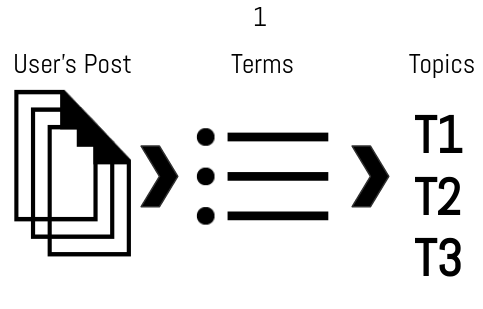
\includegraphics[scale=.5]{figs/method_1.png}
    \hspace{.5cm}
    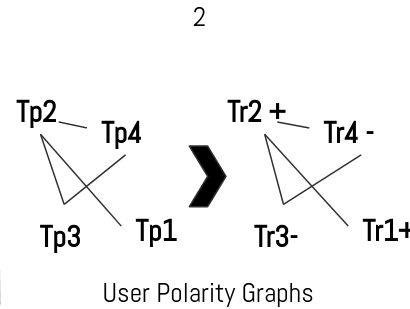
\includegraphics[scale=.5]{figs/method_2.png}\\
    \vspace{.2cm}
    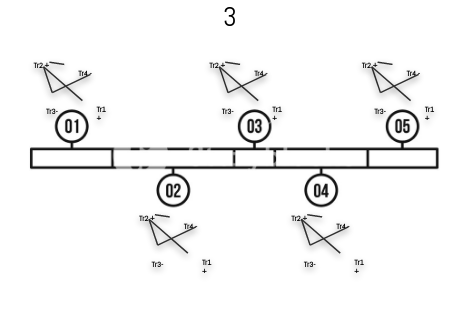
\includegraphics[scale=.6]{figs/method_3.png}
    \caption{Workflow stages for the proposed methodology}
    \label{fig:my_label}
\end{figure}

As most of the presented articles in Chapter \ref{cap:rev_literatura}, we also intend to apply text analysis over the datasets, specifically the technique that we want to employ is topic identification. Based on the work of \cite{Nolasco2016}, we aim to first identify what are the main topics of each user in a social media platform. 
After the topics identification, for each user, we could map the terms into a polarity graph. 
The polarity graph could help to identify if the most used words and terms of a user tend to be positive or negative. Related work has shown that depressive people used to manipulate more negative words. This reflects the low self-vision that this group express of themselves.
With the polarity graphs of each user, in third stage we intend to analyze how these graph have evolved over the time. In this manner, we could be capable to check if someone discourse has been turned into more positive or negative.
This could help to better explain the phenomena of depression inside social media. The time series analysis seems to be important, given that someone is considered depressed if he has manifested a set of symptoms for a certain period of time.
Also, with the graph of topics, we can apply social network metrics to understand how the users are connected, and how the people around them are affected by their discourse or behavior.

In the psychological approach, we intend to apply well defined questionnaires from psychometrics area on users selected from the computational approach. 
Psychometrics represent the theory and technique of measuring mental processes and it is applied in the fields of psychology and education. These questionnaires could be incorporated to social media users to corroborate the classification of potential users with depression.

\section{Expected Contributions}

This work still in development of methodology, with some ideas of analysis that could be made. 
The expected contributions are related to computer science and psychology.
For the computer science, we expect that employing computational metrics like social network analysis and topic classification could support people to acquire a more proper understanding of how the phenomena of depression happen in social media, and also how the social media reflects the real life. 
For the health research point of view (psychology, medicine), our approach could improve how the diagnosis of depression is performed. This could aid people with few resources to enjoy a better health by the use of technology.
\chapter{Research Methodology}\label{cap:methodology}

%A natureza da pesquisa sugere a necessidade de aproximar a teoria da prática. Como o trabalho tem como objetivo a construção de artefatos para aprimorar as relações em um ambiente de agentes inovadores, o processo investigativo deve conjugar esforços teóricos-metodológicos com a utilidade prática identificada para a sociedade.


%A condução de pesquisas requer um rigor científico e modelo a ser seguido para assegurar que sejam implementados os passos sistemáticos para explicar, descrever, explorar ou predizer fenômenos e suas relações. Esta conduta possibilita a replicação das etapas da pesquisa e facilita a condução de experimentos complementares.


\chapter{Conclusão}\label{cap6}

Contudo, esta pesquisa limita-se a tratar do diagnóstico e monitoramento das parcerias para auxiliar no balanceamento e manutenção da comunidade. Desta forma, o presente trabalho busca compreender as seguintes características: 

\begin{itemize}
	\item Recursos e Competências disponíveis;
	\item Relações de Influência e Poder; 
	\item Relevância de Participantes;
	\item Confiança de Participantes
\end{itemize}

Não fazem parte do escopo deste trabalho a proposição de mecanismos de recomendação, diagnóstico de parcerias ou análise estratégica do ecossistema. Contudo, espera-se que a plataforma e o método que serão produzidos através deste projeto de pesquisa possam fomentar o desenvolvimento de outros trabalhos nesta linha. 



%\chapter{Estado da Arte}\label{cap:estArte}

\lipsum[34]

\section*{Trabalhos Relacionados a Isto}\label{sec:primTrab}
\addcontentsline{toc}{section}{Trabalhos Relacionados a Isto}

\lipsum[34-36]
%\chapter{Materiais e Métodos}\label{cap:ferramentas}

\lipsum[43-45]

\section{Considerações Finais}

\lipsum[23]


% PARTE
%\part{Proposta}
%\chapter{Sistema Proposto}\label{cap:proposta}

Esse trabalho propõe um sistema de... 


\section{Primeira Parte do Sistema Proposto}

\lipsum[67]

\section{Considerações Finais}

\lipsum[68]


% PARTE
%\part{Parte Final}
%\include{capitulos/resultados}
%\chapter*{Conclusões e Trabalhos Futuros}\label{cap:conclusao}
\addcontentsline{toc}{chapter}{Conclusão e Trabalhos Futuros}

\lipsum[81]

\section*{Conclusões}

\lipsum[82-84]

\section*{Trabalhos Futuros}

\lipsum[85] 

% ----------------------------------------------------------
% ELEMENTOS PÓS-TEXTUAIS (Referências, Glossário, Apêndices)
% ----------------------------------------------------------
\postextual

% Referências bibliográficas
\bibliography{bibliografia}

% Glossário (Consulte o manual)
%\glossary

% Apêndices
%% ----------------------------------------------------------
% Apêndices
% ----------------------------------------------------------

% ---
% Inicia os apêndices
% ---
\begin{apendicesenv}

% Imprime uma página indicando o início dos apêndices
\partapendices

% ----------------------------------------------------------
\chapter{Trabalhos}
\label{shortpaperEISI2017}
% ----------------------------------------------------------
\begin{itemize}
	\item \textit{Shorpaper}: ESCALFONI, R. E. L., IRINEU, M. A. S and OLIVEIRA, J. \textquotedblleft Impacto das Redes de Negócios para Startups: Um Estudo Empírico na IETEC/CEFET-RJ\textquotedblright Encontro de Inovação em Sistemas de Inovação - SBSI 2017, Lavras, MG.
	\item \textit{Full paper}: ESCALFONI, R. E. L., FRANÇA, T. C., IRINEU, M. A. S., VIVACQUA, A. S., OLIVEIRA, J. \textquotedblleft Um Método para Apoiar a Identificação de Interesses entre Participantes de Ecossistemas de Startups\textquotedblright \textit{Trabalho submetido para a trilha principal do SBSI 2018.}
	\item \textit{Full paper}: MAMEDE, K. O. B., ESCALFONI, R. E. L., OLIVEIRA, J. \textquotedblleft Investigando Relações de Parceria em Ecossistemas de Startups: um estudo de caso da REINC\textquotedblright \textit{Trabalho em andamento.}

\end{itemize}
\\







%--------------------------------------------------------
\end{apendicesenv}
% ---

% Anexos
% % ----------------------------------------------------------
% Apêndices
% ----------------------------------------------------------

% ---
% Inicia os anexos
% ---
\begin{anexosenv}

% Imprime uma página indicando o início dos anexos
\partanexos

% ---
\chapter{Artigo EISI 2017}

%% This is "sig-alternate.tex" V2.1 April 2013
% This file should be compiled with V2.5 of "sig-alternate.cls" May 2012
%
% This example file demonstrates the use of the 'sig-alternate.cls'
% V2.5 LaTeX2e document class file. It is for those submitting
% articles to ACM Conference Proceedings WHO DO NOT WISH TO
% STRICTLY ADHERE TO THE SIGS (PUBS-BOARD-ENDORSED) STYLE.
% The 'sig-alternate.cls' file will produce a similar-looking,
% albeit, 'tighter' paper resulting in, invariably, fewer pages.
%
% ----------------------------------------------------------------------------------------------------------------
% This .tex file (and associated .cls V2.5) produces:
%       1) The Permission Statement
%       2) The Conference (location) Info information
%       3) The Copyright Line with ACM data
%       4) NO page numbers
%
% as against the acm_proc_article-sp.cls file which
% DOES NOT produce 1) thru' 3) above.
%
% Using 'sig-alternate.cls' you have control, however, from within
% the source .tex file, over both the CopyrightYear
% (defaulted to 200X) and the ACM Copyright Data
% (defaulted to X-XXXXX-XX-X/XX/XX).
% e.g.
% \CopyrightYear{2007} will cause 2007 to appear in the copyright line.
% \crdata{0-12345-67-8/90/12} will cause 0-12345-67-8/90/12 to appear in the copyright line.
%
% ---------------------------------------------------------------------------------------------------------------
% This .tex source is an example which *does* use
% the .bib file (from which the .bbl file % is produced).
% REMEMBER HOWEVER: After having produced the .bbl file,
% and prior to final submission, you *NEED* to 'insert'
% your .bbl file into your source .tex file so as to provide
% ONE 'self-contained' source file.
%
% ================= IF YOU HAVE QUESTIONS =======================
% Questions regarding the SIGS styles, SIGS policies and
% procedures, Conferences etc. should be sent to
% Adrienne Griscti (griscti@acm.org)
%
% Technical questions _only_ to
% Gerald Murray (murray@hq.acm.org)
% ===============================================================
%
% For tracking purposes - this is V2.0 - May 2012

\documentclass{sig-alternate-05-2015}

\hyphenation{a-tu-al com-pe-ti-ti-vi-da-de di-fe-ren-ci-ais res-pos-tas co-nhe-ci-men-to i-de-a-li-za-do-res ca-mi-nho a-tra-vés ne-gó-cio 
re-fe-rên-cias ques-ti-o-ná-rios u-ma re-si-den-tes coo-pe-ra-ção
ca-rac-te-ri-za-ção e-co-no-mia con-si-de-rar }
\begin{document}

% Copyright
\setcopyright{acmcopyright}
%\setcopyright{acmlicensed}
%\setcopyright{rightsretained}
%\setcopyright{usgov}
%\setcopyright{usgovmixed}
%\setcopyright{cagov}
%\setcopyright{cagovmixed}


% DOI
%\doi{10.475/123_4}

% ISBN
%\isbn{123-4567-24-567/08/06}

%Conference
\conferenceinfo{SBSI 2017}{June 5$^{th}$ -- 8$^{th}$, 2017, Lavras, Minas Gerais, Brazil}

%\acmPrice{\$15.00}

%
% --- Author Metadata here ---
%\conferenceinfo{WOODSTOCK}{'97 El Paso, Texas USA}
%\CopyrightYear{2007} % Allows default copyright year (20XX) to be over-ridden - IF NEED BE.
%\crdata{0-12345-67-8/90/01}  % Allows default copyright data (0-89791-88-6/97/05) to be over-ridden - IF NEED BE.
% --- End of Author Metadata ---

\title{Impacto das Redes de Negócios para Startups: \\Um Estudo Empírico na IETEC/CEFET-RJ}
\subtitle{Alternative Title: The Impact of Business Networks for Startups: An Empirical Study at IETEC/CEFET-RJ}
%
% You need the command \numberofauthors to handle the 'placement
% and alignment' of the authors beneath the title.
%
% For aesthetic reasons, we recommend 'three authors at a time'
% i.e. three 'name/affiliation blocks' be placed beneath the title.
%
% NOTE: You are NOT restricted in how many 'rows' of
% "name/affiliations" may appear. We just ask that you restrict
% the number of 'columns' to three.
%
% Because of the available 'opening page real-estate'
% we ask you to refrain from putting more than six authors
% (two rows with three columns) beneath the article title.
% More than six makes the first-page appear very cluttered indeed.
%
% Use the \alignauthor commands to handle the names
% and affiliations for an 'aesthetic maximum' of six authors.
% Add names, affiliations, addresses for
% the seventh etc. author(s) as the argument for the
% \additionalauthors command.
% These 'additional authors' will be output/set for you
% without further effort on your part as the last section in
% the body of your article BEFORE References or any Appendices.

\numberofauthors{3} %  in this sample file, there are a *total*
% of EIGHT authors. SIX appear on the 'first-page' (for formatting
% reasons) and the remaining two appear in the \additionalauthors section.
%
\author{
% You can go ahead and credit any number of authors here,
% e.g. one 'row of three' or two rows (consisting of one row of three
% and a second row of one, two or three).
%
% The command \alignauthor (no curly braces needed) should
% precede each author name, affiliation/snail-mail address and
% e-mail address. Additionally, tag each line of
% affiliation/address with \affaddr, and tag the
% e-mail address with \email.
%
% 1st. author
\alignauthor
Rafael E. L. Escalfoni\\
       \affaddr{CEFET-RJ Nova Friburgo}\\
       \affaddr{Av. Gov. R. Silveira, 1900}\\
       \affaddr{Nova Friburgo, RJ, Brasil}\\
       \email{{\large rafael.escalfoni@cefet-rj.br}}
% 2nd. author
\alignauthor
Marcelo A. S. Irineu\\
       \affaddr{CEFET-RJ Maracanã}\\
       \affaddr{Av. Maracanã, 151}\\
       \affaddr{Rio de Janeiro, RJ, Brasil}\\
       \email{{\large marcelo.irineu@cefet-rj.br}}
% 3rd. author
\alignauthor 
Jonice Oliveira\\
       \affaddr{PPGI - UFRJ}\\
       \affaddr{CCMN, Cidade Universitária}\\
       \affaddr{Rio de Janeiro, RJ, Brasil}\\
       \email{{\large jonice@dcc.ufrj.br}}
%\and  % use '\and' if you need 'another row' of author names
% 4th. author
%\alignauthor Lawrence P. Leipuner\\
%       \affaddr{Brookhaven Laboratories}\\
%      \affaddr{Brookhaven National Lab}\\
%     \affaddr{P.O. Box 5000}\\
%       \email{lleipuner@researchlabs.org}
% 5th. author
%\alignauthor Sean Fogarty\\
%       \affaddr{NASA Ames Research Center}\\
%       \affaddr{Moffett Field}\\
%       \affaddr{California 94035}\\
%       \email{fogartys@amesres.org}
% 6th. author
%\alignauthor Charles Palmer\\
%       \affaddr{Palmer Research Laboratories}\\
%       \affaddr{8600 Datapoint Drive}\\
%       \affaddr{San Antonio, Texas 78229}\\
%       \email{cpalmer@prl.com}
}
% There's nothing stopping you putting the seventh, eighth, etc.
% author on the opening page (as the 'third row') but we ask,
% for aesthetic reasons that you place these 'additional authors'
% in the \additional authors block, viz.
%\additionalauthors{Additional authors: John Smith (The Th{\o}rv{\"a}ld Group,
%email: {\texttt{jsmith@affiliation.org}}) and Julius P.~Kumquat
%(The Kumquat Consortium, email: {\texttt{jpkumquat@consortium.net}}).}
\date{30 July 1999}
% Just remember to make sure that the TOTAL number of authors
% is the number that will appear on the first page PLUS the
% number that will appear in the \additionalauthors section.

\maketitle

\begin{resumo}
As \textit{startups} têm ganhado papel de destaque no cenário atual devido a seu desempenho para o lançamento de inovações com baixo custo e risco. Contudo, para assegurar o sucesso desses empreendimentos é necessário estabelecer um ambiente colaborativo para incentivar e dar suporte às atividades. Compreender e sistematizar tais requisitos do ecossistema de \textit{startups} é fundamental para estabelecer maior capacidade competitiva. O presente artigo apresenta um estudo empírico dos aspectos das diferentes estruturas de colaboração na incubadora IETEC CEFET-RJ. 
\end{resumo}

%%%%%%
% Use esse comando apenas se o artigo for em Português
%%%%%%
\palavraschave{Ecossistemas de \textit{Startups}; redes de negócios; inovação.}

\begin{abstract}
Startups companies have prominent role in the current business scenario. This is because they can get innovation with reduced costs and risks. However, to ensure the success of these ventures it is necessary to establish a collaborative environment to encourage and support those activities. Understanding and systematizing such startup ecosystem requirements is critical to establishing greater competitive capacity. This paper presents an empirical study of different structures of the collaboration aspects in incubator IETEC CEFET-RJ.
\end{abstract}


%
% The code below should be generated by the tool at
% http://dl.acm.org/ccs.cfm
% Please copy and paste the code instead of the example below. 
%
\begin{CCSXML}
<ccs2012>
	<concept>
		<concept_id>10002951.10003227.10003241.10003243</concept_id>
		<concept_desc>Information systems~Expert systems</concept_desc>
		<concept_significance>500</concept_significance>
	</concept>
	<concept>
		<concept_id>10002951.10003260.10003282.10003292</concept_id>
		<concept_desc>Information systems~Social networks</concept_desc>
		<concept_significance>300</concept_significance>
	</concept>
</ccs2012>  
\end{CCSXML}

\ccsdesc[500]{Information systems~Expert systems}
\ccsdesc[300]{Information systems~Social networks}


%
% End generated code
%

%
%  Use this command to print the description
%
\printccsdesc

% We no longer use \terms command
%\terms{Theory}

\keywords{Startup Ecosystem; business networking;  innovation}

\section{Introdução}
\textit{Startups} são empreendimentos associados à inovação e tecnologia que vêm ganhando papel de destaque no cenário atual em função da flexibilidade do modelo de negócios, baixos investimentos iniciais e maior dinamicidade nos ciclos de transferência tecnológica \cite{ries-2011}. Esta estrutura de negócios exerce  um papel fundamental no lançamento de novos produtos em um ambiente no qual a complexidade tem aumentado consideravelmente e despertado a necessidade de buscar novas estratégias para geração de inovações e diferenciais competitivos \cite{hardwick-et-al-2013}.

O estabelecimento de parcerias é essencial para a geração de inovações, pois o sucesso depende de um conjunto de infraestruturas e capacidades que abarcam desde a concepção do produto até a comercialização e distribuição no mercado. Além disso, a colaboração entre organizações é uma importante forma de lidar com as incertezas e riscos inerentes ao processo de inovação \cite{chesbrough-appleyard-2007, west-bogers-2014}. Frequentemente, empresas consolidadas não controlam esses ativos complementares, e, no caso das \textit{startups}, tal necessidade fica mais latente \cite{candido-souza-15}. 

As \textit{startups} têm maiores chances de sucesso quando se estabelecem em ecossistemas empreendedores, que estimulem o desenvolvimento de negócios e inovações \cite{spigel-2015}. Os ecossistemas de \textit{startups} são núcleos tecnológicos, onde parceiros compartilham recursos e habilidades específicas, através de apoio mútuo para estabelecer maior capacidade de competitividade em um cenário maior \cite{cukier-et-al-2015}. Desta forma, entender como tais relações de parcerias entre atores do ecossistema é crítico tanto da empresa quanto do próprio ambiente. O presente artigo apresenta um estudo feito na incubadora tecnológica do CEFET-RJ, a IETEC, onde foram identificados aspectos de colaboração entre os diferentes atores participantes deste ambiente de negócios, destacando os principais recursos compartilhados e auxiliando na identificação das características dos relacionamentos entre empreendedores. 

O restante deste artigo está organizado da seguinte forma: a Seção 2 apresenta os conceitos que fundamentam este trabalho. A Seção 3 detalha a caracterização da pesquisa - a elaboração do questionário utilizado, da IETEC e perfil dos entrevistados. A Seção 4 traz uma discussão sobre as respostas obtidas. Na Seção 5 são apresentadas as conclusões da pesquisa e os trabalhos futuros.\\


\section{Fundamentação Teórica}
\subsection{{\subsecit Startups}}
O termo \textquotedblleft startup\textquotedblright\ é utilizado para designar uma instituição temporária formada com o intuito de validar conceitos até que se tenha as condições mínimas para operacionalizar uma empresa, um projeto de organização que visa identificar um modelo de negócio consolidado e que possa ser expandido \cite{blankdorf-12}. Caso não haja sucesso em encontrar este caminho, a natureza do empreendimento permite interrompê-lo sem maiores prejuízos aos colaboradores e demais envolvidos, o que permite enfrentar maiores riscos e incertezas \cite{ries-2011}.

As novas ferramentas e metodologias de desenvolvimento, como o movimento \textit{Lean Startup}, propõem uma metodologia de experimentação e aprendizagem interativa. Seu ciclo de vida envolve um conjunto de passos que engloba desde o desenvolvimento de um conceito até o estabelecimento do negócio. Segundo Santos \cite{santos-2015}, as ações podem ser agrupadas nas seguintes fases: 

\begin{itemize}
	\item \textbf{Descoberta}: agrupa as ações para validar as hipóteses formuladas e para verificar se a solução ataca um problema relevante que consiga atrair o interesse das pessoas; 
	\item \textbf{Validação}: uma vez que o problema fica bem definido na etapa anterior, busca-se conhecer o segmento de clientes dispostos a pagar pelo produto. São feitos os ajustes necessários para tornar o produto rentável. Por vezes, recorre-se a ajustes para atender melhor às necessidades, estratégia conhecida como pivotagem.
	\item \textbf{Criação do Cliente}: até este ponto, o produto já foi desenvolvido e seu público-alvo já está bem definido. A criação do cliente está relacionada com a massificação do produto e a fidelização, o esforço para popularizar a marca. 
	\item \textbf{Construção da Empresa}: este estágio é a consolidação do empreendimento, quando a \textit{startup} se torna um negócio. Há uma estruturação da organização, com a definição dos papéis e responsabilidades.
\end{itemize}

Este tipo de empreendimento, tem sido tratado com grande expectativa por conta de seu potencial para o lançamento de inovações disruptivas \cite{weiblen-chesbrough-2016}. Devido a sua dinâmica, os custos de lançamento de produtos tornaram-se muito menores, trazendo à tona outros fatores de maior importância como por exemplo a inventividade e conhecimento de seus idealizadores e maior tolerância a riscos. 

Como forma de viabilizar tais negócios, um número crescente de instituições de apoio tem se estabelecido para orientar o negócio nos seus primeiros dias. São investidores e capitalistas de risco, incubadoras e aceleradoras, além de órgãos governamentais de suporte -- atores que compõem os ecossistemas de startups, provendo infraestrutura, espaço de mercado, parcerias consolidadas e processos estabelecidos~\cite{anthony-12}.

\subsection{Ecossistemas de {\subsecit Startups}}

Ecossistema de \textit{startups} são arranjos de atores (empreendedores, apoiadores, universidades, dentre outros) que buscam estabelecer os meios necessários para lançar novos produtos no mercado \cite{torres-souza-2016}. Essa comunidade funciona de maneira harmônica e dinâmica, tal qual um ecossistema biológico, onde o meio está constantemente se adaptando às mudanças, como  quando ocorre extinção de algum componente \cite{torres-souza-2016}. 

A rede de negócios é um dos aspectos principais para o cenário das \textit{startups}. O compartilhamento de ideias, experiências entre empreendedores novatos e experientes auxilia no aprendizado e desenvolvimento de competências essenciais para o sucesso de empresas. As conexões com organizações de suporte, como universidades e órgãos de fomento permitem acesso a recursos complementares para o desenvolvimento de produtos, tais como tecnologias e linhas de financiamento \cite{isenberg-2011} \cite{motoyama-waltins-2014} \cite{torres-souza-2016}. 

Para assegurar o equilíbrio e, consequentemente seu êxito em apoiar \textit{startups}, diferentes tipos de parcerias devem ser firmadas. Motoyama e Watkins \cite{motoyama-waltins-2014} estabelecem quatro conexões chaves para o ecossistema de \textit{startups}, são elas:

\begin{itemize}
	\item \textbf{Conexões entre empreendedores}: estabelecem uma comunidade de aprendizagem, onde as interações possibilitam a troca de saberes entre empreendedores com diferentes níveis de experiência. Os \textit{feedbacks} obtidos por meio deste tipo de rede proporcionam um  meio de aprendizado fundamental sobre o negócio.
	\item \textbf{Conexões entre organizações de suporte}: compreendem as relações estratégicas e funcionais entre instituições de pesquisa, universidades, incubadoras, dentre outras. Determinam o direcionamento dado ao ecossistema através da promoção de temas de interesse e no suporte de empreendimentos relacionados.
	\item \textbf{Conexões entre empreendedores e principais organizações de apoio}: Representam as parceiras firmadas entre \textit{startups} e as organizações de suporte. 
	\item \textbf{Demais conexões de apoio}: Evidenciam outros arranjos existentes entre empreendedores e atores diversos, como mentores, fornecedores e demais empresas parceiras.

\end{itemize}

\section{Abordagem Metodológica}
O presente estudo recorreu a evidências baseadas na experiência de especialistas com diferentes perspectivas de um ecossistema de \textit{startups}. Participaram através de questionários e entrevistas três gestores de empresas intensivas em conhecimento, um representante de um órgão de fomento e o coordenador de incubadora. 

No centro da aplicação do estudo encontra-se a IETEC -- a incubadora de empresas tecnológicas do CEFET-RJ. Fundada em 1994 com a proposta de apoiar empreendimentos na área de telecomunicação, desenvolvimento de \textit{hardware} e \textit{software}, a instituição passou por uma reformulação em 2010, passando a contemplar projetos tecnológicos e inovadores de todas as áreas de conhecimento mantidas pelo CEFET-RJ. Atualmente, a IETEC possui 8 projetos residentes, além de ter contribuído para a graduação de 18 empresas com um faturamento médio de R\$ 6,5 milhões. 

\subsection{Processo Investigativo}
%As entrevistas foram apoiadas por roteiros semiestruturados, constituídos de perguntas principais baseadas nas dimensões propostas por Motoyama e Watkins \cite{motoyama-waltins-2014} que evidenciam a relevância de diferentes tipos de redes de negócios dentro do ecossistema, sobretudo as conexões entre empreendedores e demais participantes do ambiente de negócios, dentro e fora da incubadora. Foram elaboradas questões abertas que buscavam identificar como as parcerias são formadas, como são prospectadas pelos gestores, se as startups contam com um processo de montar e manter suas parcerias, que tipo de recurso é intercambiado. Buscamos também medir o grau de influência nos negócios a partir de cada parceria, da relevância da incubadora, no mercado.

As entrevistas foram apoiadas por roteiros semiestruturados, constituídos de perguntas principais baseadas nas dimensões propostas por Motoyama e Watkins \cite{motoyama-waltins-2014} que evidenciam a relevância de diferentes conexões dentro do ecossistema, sobretudo as interações entre empreendedores e demais participantes do ambiente de negócios, dentro e fora da incubadora. 

Para isto, foram elaboradas questões abertas que buscavam caracterizar o ecossistema e identificar a relevância das relações: 
\begin{enumerate}
	\item \textbf{Conexões entre empreendedores: }(a) Quem são os principais parceiros? (b) O que leva a buscar cooperação? (c) Como são formadas e mantidas as parcerias? Há um processo formal de identificação de colaboradores? (d) Que tipo de recurso é compartilhado? (e) Que critérios são adotados para aceitação de parceiros? 
	
	\item \textbf{Conexões entre empreendedores e principais organizações de apoio: } (a) Quais as principais motivações para buscar apoio de instituições de suporte? (b) Quais são as organizações de fomento mais importantes para o seu negócio? (c) Como tais órgãos têm auxiliado o seu negócio? 
	
	\item \textbf{Demais conexões de apoio: } (a) Seu negócio mantém vínculos com outras organizações? (b) Qual é o papel destas parcerias? 
	
	\item \textbf{Conexões entre organizações de suporte:} (a) Possui parcerias com outros órgãos de apoio (quais)? (b) O que se busca neste tipo de parceria? (c) Como funcionam tais conexões?
\end{enumerate}

O tratamento de dados foi feito utilizando o método de Análise de Conteúdo, no qual buscou-se identificar padrões que possam surgir dos documentos analisados \cite{bardin-09}. O processo de análise foi conduzido em 3 etapas: 

\begin{itemize}
	\item \textbf{Pré-análise}: em um primeiro momento, o material das entrevistas e dos questionários foi organizado através de uma categorização. Para isto, as questões foram divididas nos seguintes assuntos principais: caracterização do agente participante, formação e prospecção de parcerias, percepção da importância de conexões formadas com empreendedores e instituições de apoio, procedimentos para a manutenção e estratégias de negócio voltadas para  as redes, papel e relevância das instituições apoiadoras para o negócio. As respostas obtidas foram separadas pelo perfil dos especialistas, levando em conta sua experiência empreendedora e o papel exercido na organização estudada.
	
	\item \textbf{Descrição analítica}: neste passo, buscou-se elucidar as opiniões a partir da construção de quadro de referências e da busca por sínteses coincidentes e ideias divergentes. Contrapomos as opiniões para identificar conflitos e então voltamos a procurar os participantes para tirar dúvidas; e 
	
	\item \textbf{Interpretação}: após tirar dúvidas, foram identificadas as conexão entre ideias e conhecimentos adquiridos ao longo do trabalho. A análise crítica destas relações e a base teórica que permeia este trabalho, formam a base das evidências empíricas deste estudo.
\end{itemize}

\section{Resultados Obtidos}
Conforme identificado pela pesquisa, as conexões entre empreendedores manifestam-se de diversas maneiras: através da trocas informais de conhecimento por meio do espaço de \textit{co-working}, por reuniões periódicas na incubadora e relações pontuais decorrentes de indicações. As interações, normalmente ocorrem para troca de experiências, para obter conhecimentos complementares ou para solucionar gargalos em processos operacionais. A literatura indica como uma das razões deste tipo de cooperação, a complementaridade da cadeia de valor \cite{candido-souza-15}. Conforme identificado, há relatos de parcerias firmadas com empresas consolidadas para este fim.

No ano passado, iniciou-se um programa de mentoria. Os projetos que participaram da dinâmica, passaram por um processo de compreensão dos propósitos de seus produtos e então foi feita a escolha do mentor mais adequado para cada caso. Empreendedores novatos passaram a se reunir com empresários experientes periodicamente por meio de videoconferências.  Este contato possibilitou melhorar a percepção do negócio, acarretando em reformulações de conceitos ou mesmo dando mais confiança ao conceito do produto. Alguns projetos montaram parcerias e conseguiram aportes financeiros e apoio por meio de consultorias. 

Com relação às conexões entre organizações de apoio, veri-ficou-se um ambiente fértil em ações para prover uma estrutura adequada para os empreendedores. A exemplo das manifestações, a IETEC está envolvida em consórcios entre incubadoras e parques tecnológicos e fóruns temáticos para promoção de inovação, onde tem participado ativamente de programas para intercâmbio de experiências. A instituição tem mantido parcerias com empresas, sobretudo as empresas graduadas, que atuam ativamente no programa de mentoria. 

O relacionamento entre empreendedores e organizações de apoio ocorre predominantemente por meio da incubadora. Porém, grande parte dos empreendedores mantém um vínculo sistemático com universidades e centros de pesquisa. O CEFET-RJ, por exemplo, possui um núcleo de inovação tecnológica, responsável por promover a inovação e transferência tecnológica, além de servir de interface da universidade com a incubadora. 

Os empreendedores têm conseguido aporte financeiro por meio de fomento. Para facilitar o acesso à informação, a IETEC tem mantido um mapeamento de editais e das políticas propostas dos órgãos de fomento. Este recurso tem sido usado para promover o alinhamento das \textit{startups} com as aspirações da Sociedade manifestadas pelas linhas de financiamento disponibilizadas.

O processo investigativo também almejou identificar as principais barreiras para a formação de parcerias. Verificou-se que a falta de planejamento é um problema recorrente, que dificulta a comunicação com os pares e a percepção de futuro para o negócio. O medo em expor as opiniões pode comprometer as relações: por vezes, o empreendedor tem receio de expor as ideias e ser plagiado - faltam mecanismos para distinguir as informações sensíveis para o negócio das que devem ser compartilhadas com os potenciais parceiros. Os problemas de comunicação dos interlocutores da \textit{startup} também foram relatados, assim como a falta de informações sobre potenciais parceiros, a falta de sinergia e problemas financeiros. 

\section{Conclusão e Trabalhos Futuros}
A inovação tem sido descrita como o único caminho para estabelecer um modelo de competividade sustentável na economia atual \cite{weiblen-chesbrough-2016}. Neste contexto, as \textit{startups} têm sido uma poderosa ferramenta de experimentação e aprendizagem, com um grande potencial para a geração de produtos com maior valor agregado. Contudo, o sucesso desse tipo de empreendimento é dependente do ecossistema no qual está inserido e das relações mantidas entre seus agentes \cite{blankdorf-12}\cite{candido-souza-15}\cite{motoyama-waltins-2014}. 

%Este artigo apresentou um estudo das ações promovidas dentro da IETEC/CEFET-RJ para criar e manter redes de parcerias entre diferentes atores do ecossistema de \textit{startups}. Conforme foi verificado, todas as conexões chaves mencionadas em Motoyama e Watkins \cite{motoyama-waltins-2014} estão sendo contempladas de alguma forma. Por outro lado, deve-se considerar o grau de sistematização das interações e a dependência dos agentes principais, sobretudo da incubadora. É preciso criar mecanismos para difundir melhor as informações sobre os recursos disponíveis na rede, a exemplo do que foi feito com o processo de acompanhamento e divulgação dos editais de fomento mencionado. Também não há um processo estruturado para a identificação e gestão da rede. Todas as atividades ocorrem de maneira \textit{ad hoc}, o que pode deixar grandes oportunidades dependentes da percepção dos envolvidos.

O presente artigo apresenta um estudo em andamento que busca compreender como ocorrem as interações entre atores de ecossistemas de \textit{startups} para aprimorá-las. Nesta primeira etapa da pesquisa, utilizou-se a IETEC/CEFET-RJ como objeto de estudo, onde foi feito um levantamento de como as relações ocorrem atualmente, vislumbrando oportunidades de aperfeiçoamento por meio de técnicas e ferramentas computacionais.

Os resultados obtidos através do estudo não podem ser generalizados, mas trazem indícios de que as conexões chaves mencionadas por Motoyama e Watkins \cite{motoyama-waltins-2014} estão sendo contempladas de alguma forma. Por outro lado, deve-se considerar o grau de sistematização das interações e a dependência dos agentes principais, sobretudo da incubadora. Não há um processo estruturado para a identificação e gestão da rede e todas as atividades ocorrem de maneira \textit{ad hoc}, o que pode deixar grandes oportunidades dependentes da percepção dos envolvidos. É preciso criar mecanismos para difundir melhor as informações sobre os recursos disponíveis na rede, a exemplo do que foi feito com o processo de acompanhamento e divulgação dos editais de fomento mencionado.

Em trabalhos futuros, esperamos ampliar nosso conhecimento acerca do universo das \textit{startups} por meio de uma análise investigativa mais detalhada. Estamos planejando um estudo envolvendo outras incubadoras, aceleradoras e outros parceiros da IETEC. Pretendemos explorar o planejamento de parcerias. O objetivo é auxiliar os participantes do ambiente empreendedor a terem uma visão mais ampla das possibilidades de parceria e promover a gestão de rede por meio de mecanismos de análise de redes sociais. Um exemplo de aplicação seria a identificação dos agentes principais da rede e os gargalos para cada participante. Também vislumbramos a utilização de sistemas de recomendação para identificar parceiros mais apropriados.


%ACKNOWLEDGMENTS are optional
\section{Agradecimentos}
Gostaríamos de agradecer à Incubadora de Empresas Tecnológicas IETEC CEFET-RJ por todo apoio ao projeto. Ao CNPq, CAPES e FAPERJ.

%
% The following two commands are all you need in the
% initial runs of your .tex file to
% produce the bibliography for the citations in your paper.
\bibliographystyle{abbrv}
\bibliography{eisi2017}  % sigproc.bib is the name of the Bibliography in this case
% You must have a proper ".bib" file
%  and remember to run:
% latex bibtex latex latex
% to resolve all references
%
% ACM needs 'a single self-contained file'!
%
%APPENDICES are optional
%\balancecolumns


\end{document}

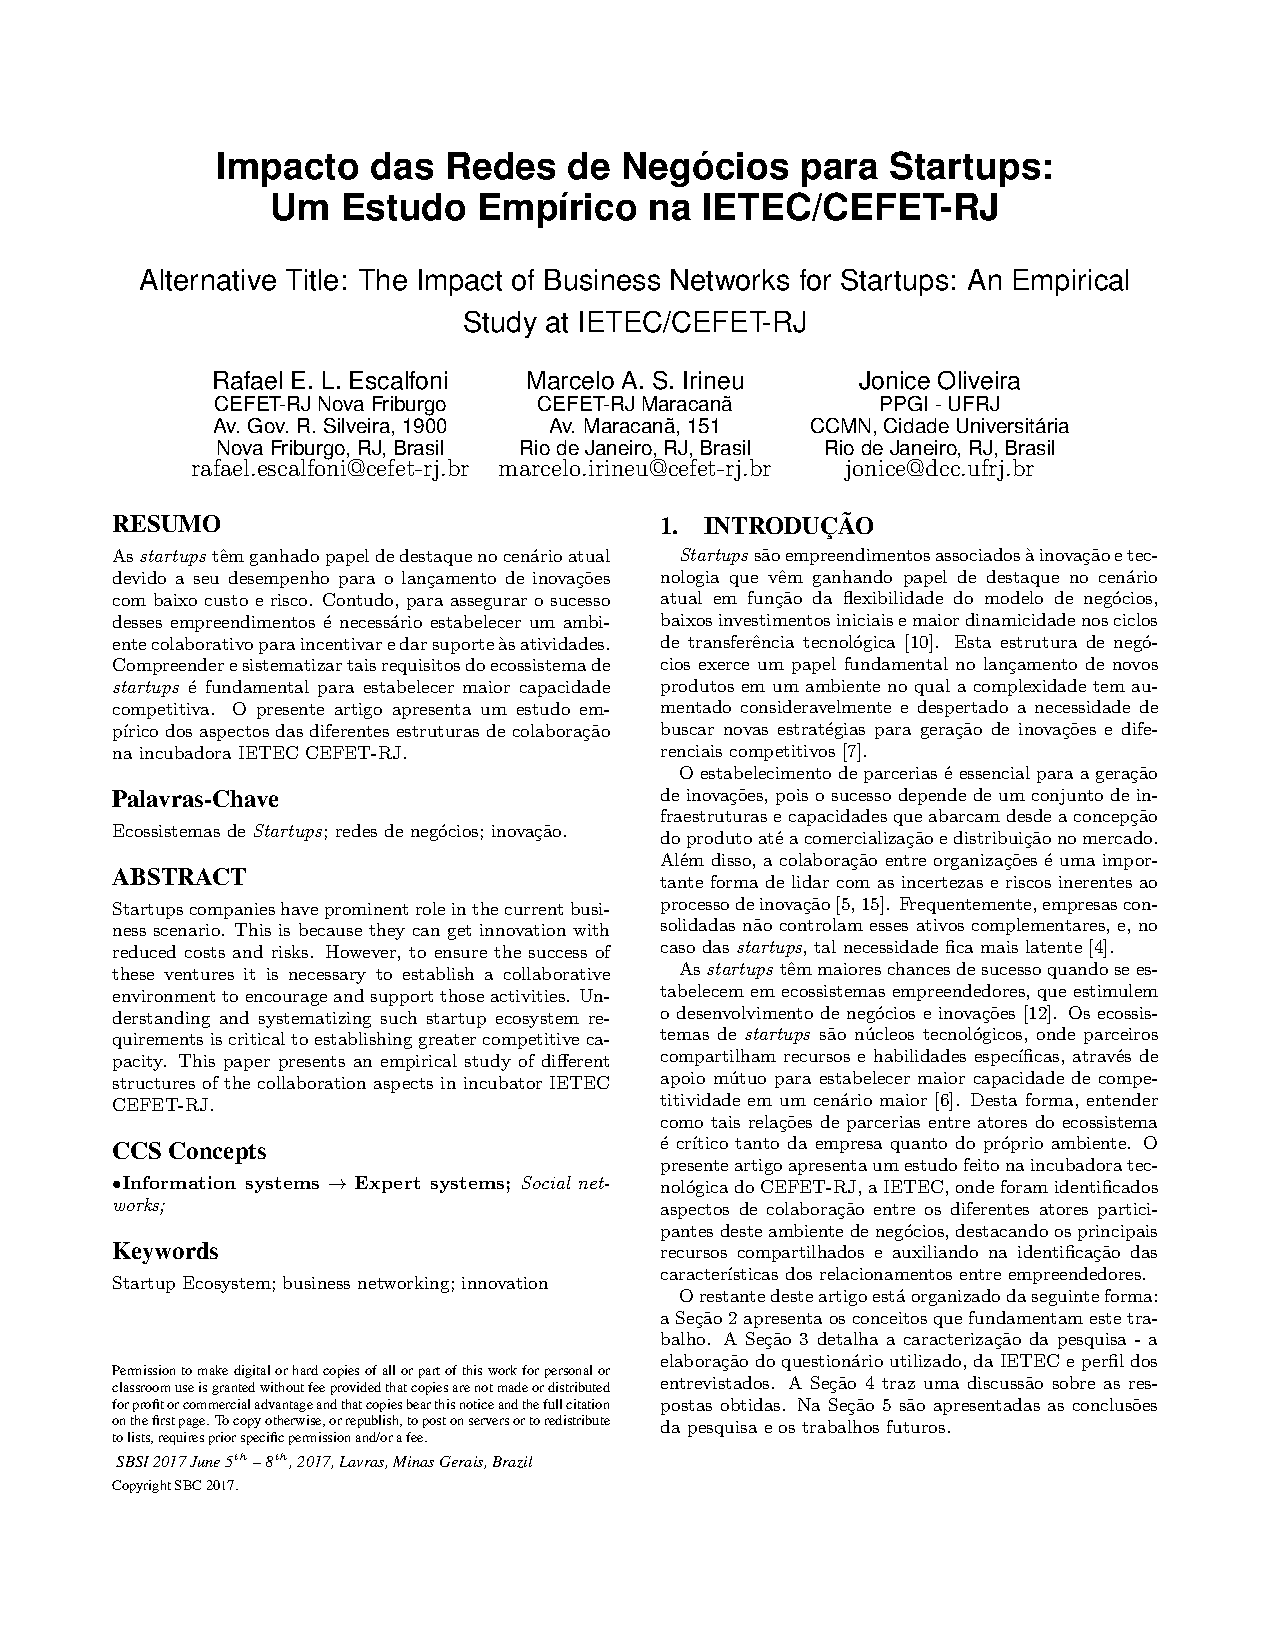
\includepdf[pages=-]{postextual/eisi2017.pdf}

% ---
\chapter{Artigo SBSI 2018}
% ---
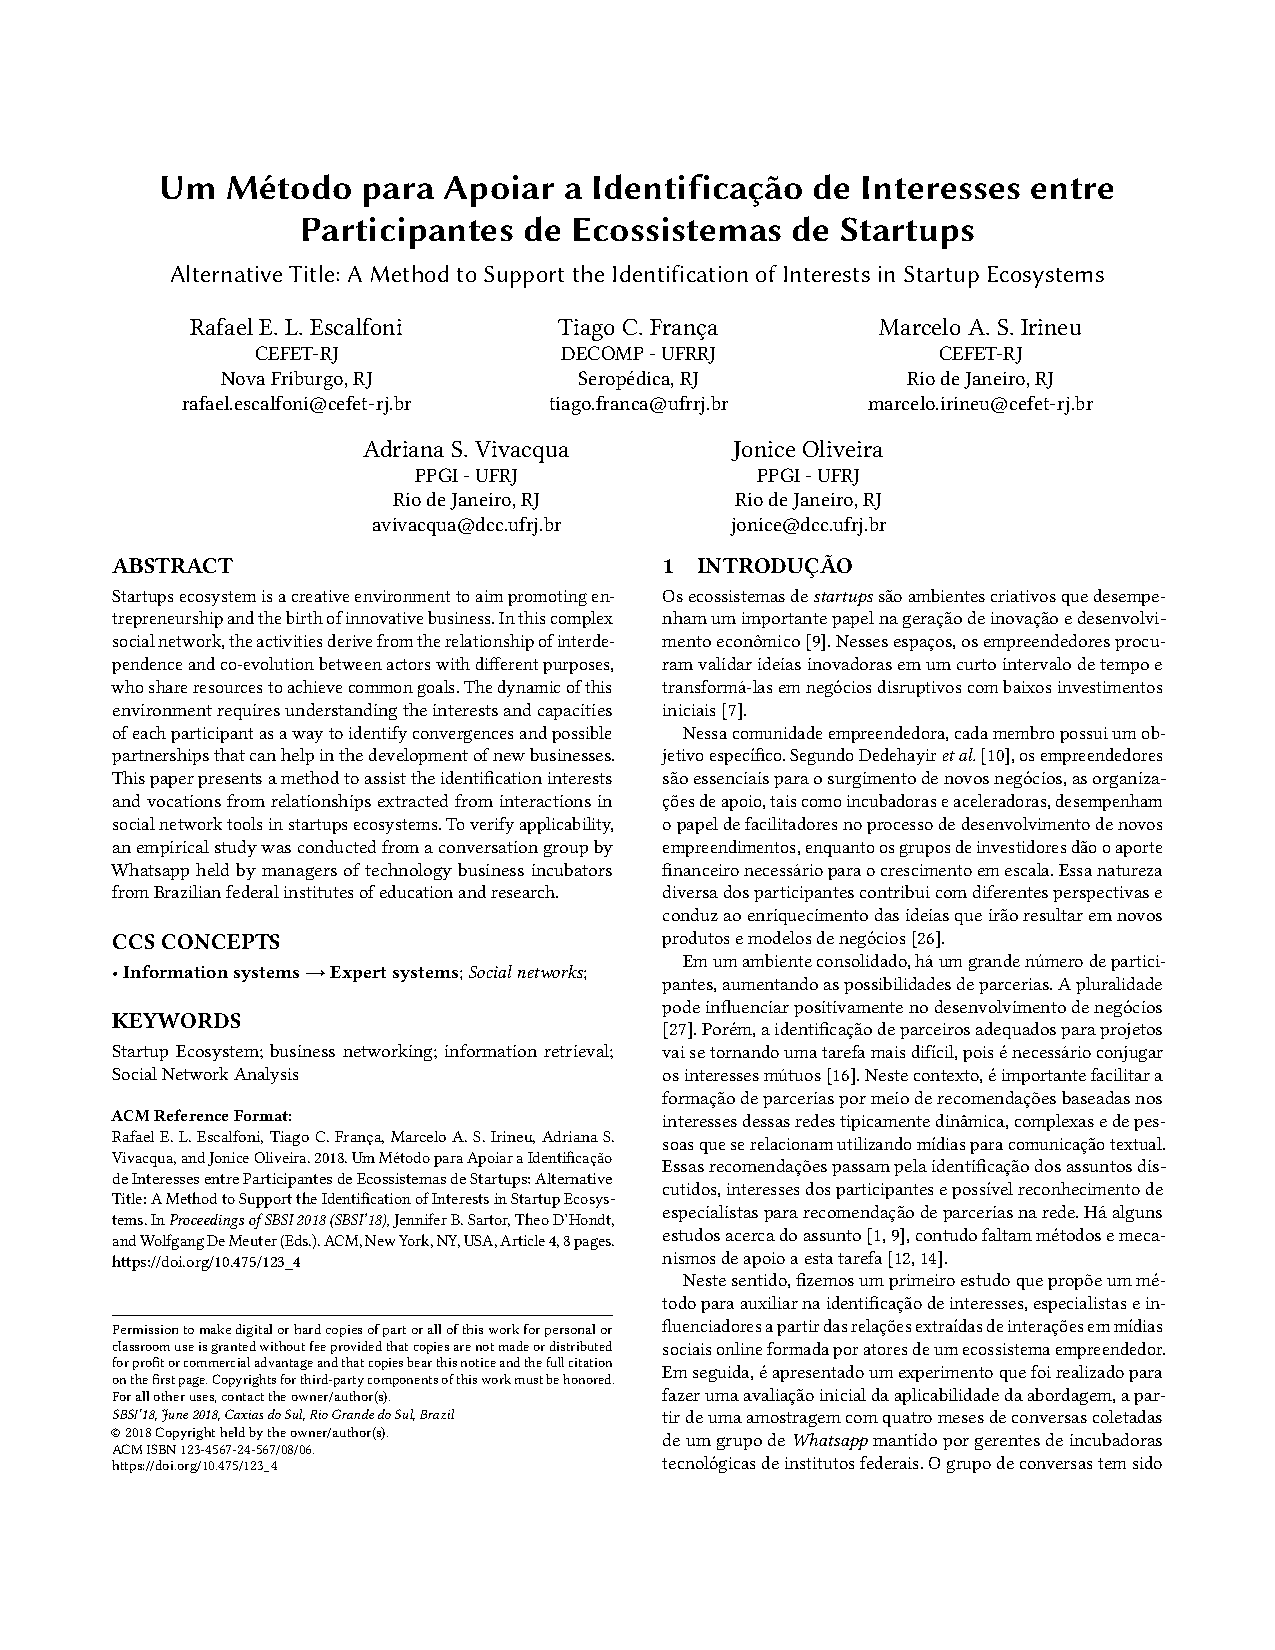
\includepdf[pages=-]{postextual/sbsi2018.pdf}

\chapter{Artigo Submetido no BIDU 2018 - Workshop on Big Social Data and Urban Computing}
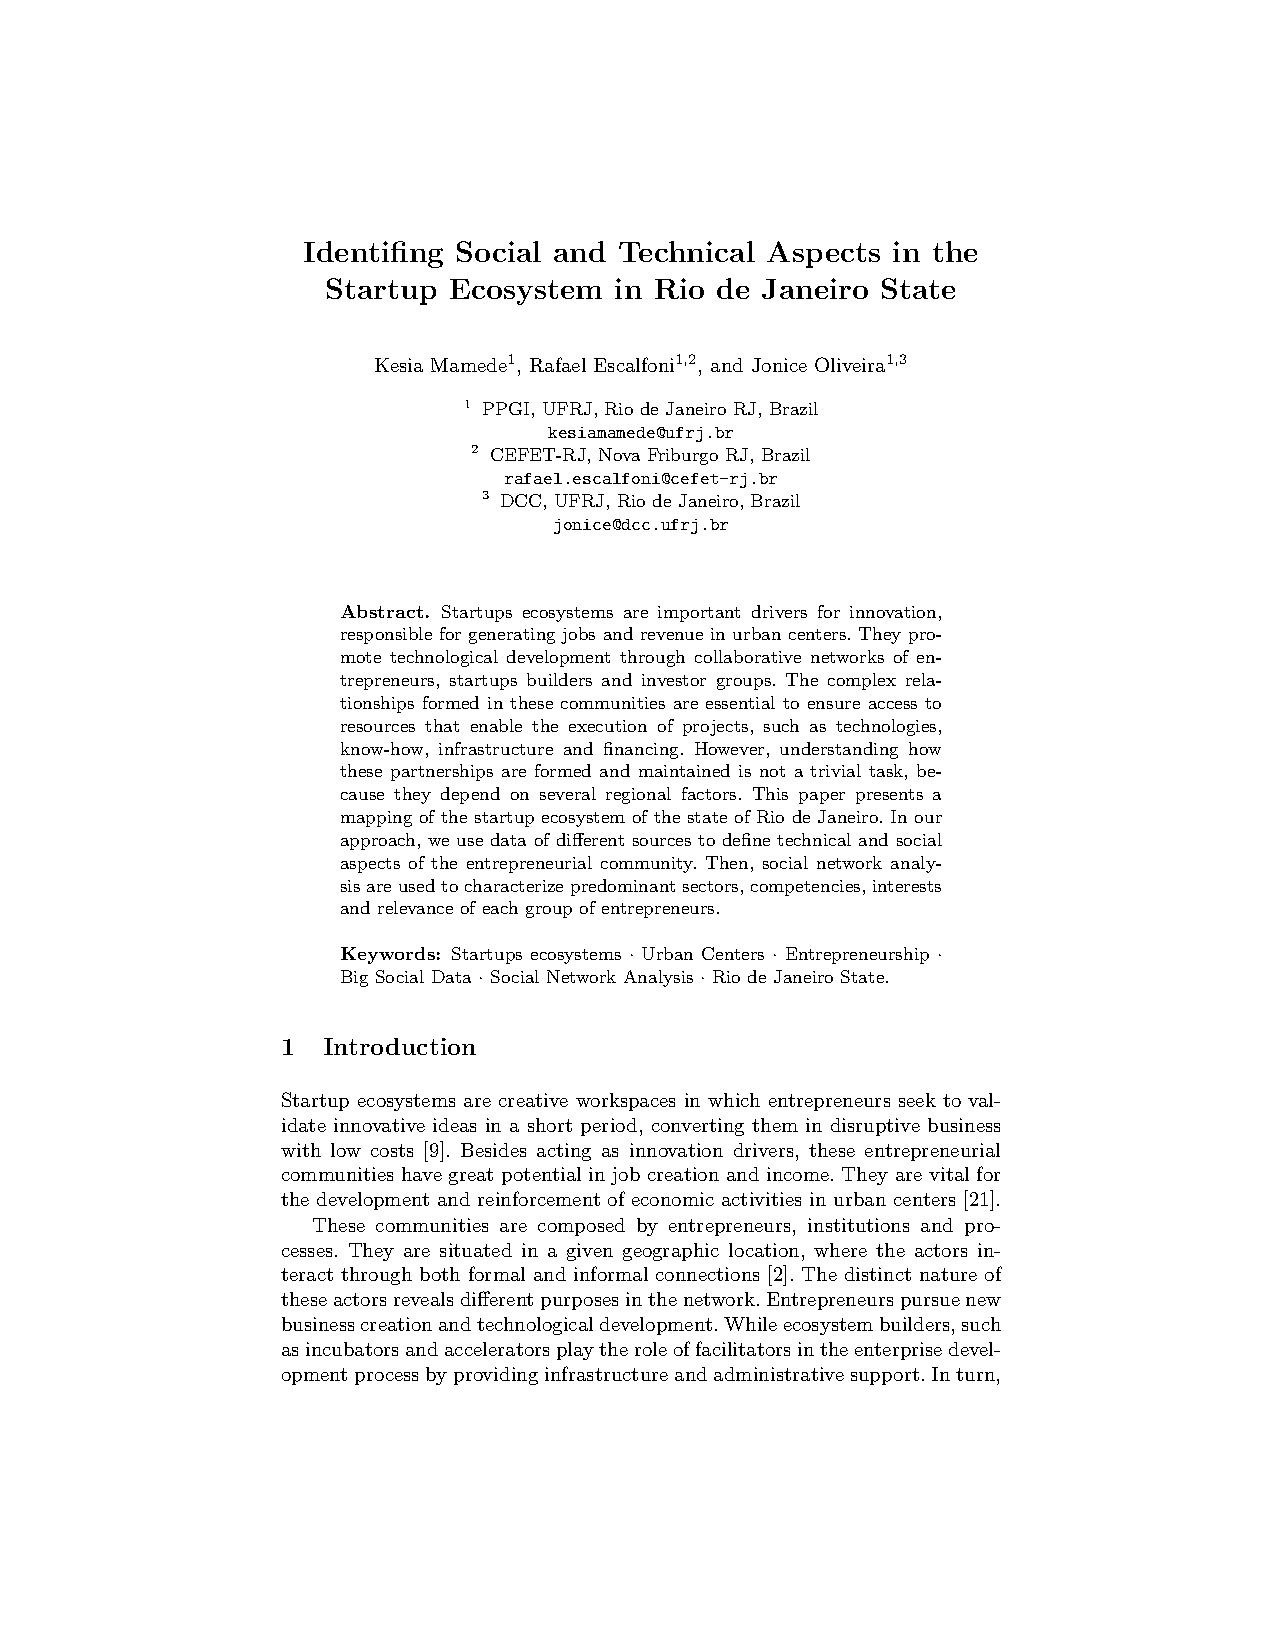
\includepdf[pages=-]{postextual/bidu_2018.pdf}

\end{anexosenv}

% Índice remissivo (Consultar manual)
%\phantompart
%\printindex

\end{document}
% * <marcosaraujo.mvma@gmail.com> 2017-04-10T12:18:58.497Z:
%
% ^.